\documentclass[12pt,a4paper]{article}

\usepackage[serbian]{babel}

\usepackage{graphicx}
\usepackage{float}

\usepackage{listings}
\usepackage{xcolor} % for setting colors

% text width and height
\textwidth 16cm
\textheight 23cm

% distance from the top
\voffset -1.5cm

% distance from the left
\hoffset 0cm
\oddsidemargin 0mm

% distance from the bottom
\footskip 1.5cm

\linespread{1}

% set the default code style
\lstset{language=python,
     xleftmargin=20pt,
      basicstyle=\ttfamily,
      morekeywords={to, downto, then},
      keywordstyle=\color{blue}\ttfamily,
      stringstyle=\color{red}\ttfamily,
      commentstyle=\color{green}\ttfamily,
      morecomment=[l][\color{magenta}]{\#},
      basicstyle=\small
}

\title{Analiza skupa podataka Food choices}
\author{Tijana Jevti\' c \\ Jelena Mrdak}

\setlength\parindent{0pt}

\newpage

\begin{document}
\maketitle

\newpage

\begin{abstract}
Skup podataka Food choices predstavlja skup odgovora studenata sa koledza na odre\dj ena pitanja vezana za njihove navike u ishrani. Dakle, podaci su dobijeni anketiranjem 125 studenata na 61 pitanje razli\v citog tipa. Neka pitanja se konkretno ti\v cu njihovih preferenca vezanih za hranu, njihovih navika, dok se kroz ostala dobija vi\v se informacija o njihovom socio-ekonomskom statusu. Sve to zajedno \v cini bogat skup podataka iz kog se moze zaklju\v citi dosta zanimljivih pravilnosti.

\v Sta dana\v snji studenti na koled\v zu najvi\v se vole da jedu? Koliko \v cesto kuvaju? Zasto jedu i da li je jedini odgovor zbog gladi? Koliko to \v sto se prejedaju i razlozi zbog kojih konzumiraju svoju omiljenu hranu uti\v u na njihovu te\v zinu?

Na ova i jo\v s mnogobrojna pitanja, poku\v sa\' cemo da odgovorimo u ovom radu koriste\' ci programski jezik python i adekvatne biblioteke.
\end{abstract}

\newpage

\tableofcontents

\newpage

\section{Opis skupa podataka}
Za po\v cetak \' cemo se povr\v sno upoznati sa skupom podataka koji se nalazi u datoteci food\_coded.csv.
\\
\begin{lstlisting}[mathescape=true]
df = pd.read_csv('./food_coded.csv', na_values="none")
print(data.shape)
\end{lstlisting}
Skup podataka je u\v citan, nedostaju\' ce vrednosti su obele\v zene sa none i izlaz je:
\begin{verbatim}
(125, 61)
\end{verbatim}
Skup se sastoji od 61 atributa i 125 redova.\\
Atribute dobijamo: 
\begin{lstlisting}[mathescape=true]
print(data.columns)
\end{lstlisting}
Spisak svih atributa:
\begin{verbatim}
Index(['GPA', 'Gender', 'breakfast', 'calories_chicken', 'calories_day',
       'calories_scone', 'coffee', 'comfort_food', 'comfort_food_reasons',
       'comfort_food_reasons_coded', 'cook', 'comfort_food_reasons_coded.1',
       'cuisine', 'diet_current', 'diet_current_coded', 'drink',
       'eating_changes', 'eating_changes_coded', 'eating_changes_coded1',
       'eating_out', 'employment', 'ethnic_food', 'exercise',
       'father_education', 'father_profession', 'fav_cuisine',
       'fav_cuisine_coded', 'fav_food', 'food_childhood', 'fries', 'fruit_day',
       'grade_level', 'greek_food', 'healthy_feeling', 'healthy_meal',
       'ideal_diet', 'ideal_diet_coded', 'income', 'indian_food',
       'italian_food', 'life_rewarding', 'marital_status',
       'meals_dinner_friend', 'mother_education', 'mother_profession',
       'nutritional_check', 'on_off_campus', 'parents_cook', 'pay_meal_out',
       'persian_food', 'self_perception_weight', 'soup', 'sports', 'thai_food',
       'tortilla_calories', 'turkey_calories', 'type_sports', 'veggies_day',
       'vitamins', 'waffle_calories', 'weight'],
      dtype='object')
\end{verbatim}

U nastavku \' cemo pomenuti svaki od atributa kako bi se \v citalac upoznao sa skupom podataka, a posebnu pa\v znju \' cemo posvetiti onima koje koristimo u istra\v zivanju.

\begin{itemize}
  \item GPA - numeri\v cki, prosek na fakultetu
  \item Pol - kategori\v cki\\
    \textbf{1} - \v zensko\\
    \textbf{2} - mu\v sko
  \item Doru\v cak - koja od 2 ponudjene slike ispitanike vi\v se asocira na doru\v cak
  \item Procena kalorija u jednom par\v cetu piletine\\
    \textbf{1} - 265\\ 
    \textbf{2} - 430\\
    \textbf{3} - 610\\
    \textbf{4} - 720
  \item Da li je bitna koli\v cina kalorija koja se konzumira dnevno\\
    \textbf{1} - ne znam koliko kalorija treba konzumirati dnevno\\
    \textbf{2} - uop\v ste nije bitno\\
    \textbf{3} - umereno je bitno\\
    \textbf{4} - veoma je bitno
  \item Procena kalorija u kola\v cu iz Starbucks-a\\
    \textbf{1} - 107 cal\\ 
    \textbf{2} - 315 cal\\ 
    \textbf{3} - 420 cal\\ 
    \textbf{4} - 980 cal
  \item Kafa - koja od 2 ponu\dj ene slike ispitanike vi\v se asocira na kafu
  \item Hrana za utehu - koja hrana asocira ispitanike na dom i lepe uspomene, \v cini ih sre\' cnim
    Ispitanici treba da navedu izmedju 3 i 5 razli\v citih jela.
  \item Za\v sto pose\v zu za hranom za utehu \\
    Ispitanici treba da navedu do 3 razloga za\v sto jedu hranu za utehu (npr. tuga, sre\' ca, bes)
  \item Hrana za utehu - kodirana\\
   \textbf{1} - stres\\
   \textbf{2} - dosada\\
   \textbf{3} - depresija\\
   \textbf{4} - glad\\
   \textbf{5} - lenjost\\
   \textbf{6} - hladno vreme \\
   \textbf{7} - sre\'  ca\\ 
   \textbf{8} - gledanje televizije\\
   \textbf{9} - ni\v sta od navedenog
   \item Kuvanje - koliko ispitanici cesto kuvaju\\
    \textbf{1} - svakog dana\\
    \textbf{2} - nekoliko dana nedeljno\\
    \textbf{3} - koliko \v cesto mogu, ali retko\\
    \textbf{4} - jedino za praznike\\
    \textbf{5} - nikada
  \item Koji tip kuhinje su jeli kad su bili mali\\
    \textbf{1} - ameri\v cka\\
    \textbf{2} - meksi\v cka/\v spanska\\
    \textbf{3} - korejska/azijska\\
    \textbf{4} - indijska\\
    \textbf{5} - ameri\v cka sa internacionalnim jelima\\
    \textbf{6} - ostalo
  \item Trenutna dijeta
  \item Trenutna dijeta - kodirano od 1 do 4
  \item Koju sliku asociraju sa picem
  \item Kako se ishrana promenila od kada su na koledzu
  \item Kako se ishrana promenila\\
    \textbf{1} - na lo\v sije\\
    \textbf{2} - na bolje\\
    \textbf{3} - isto\\
    \textbf{4} - nije sigurno
  \item Kako se ishrana promenila u terminima toga \v sta jedu
  \item Prejedanje - koliko se ispitanici \v cesto prejedaju tokom nedelje\\
    \textbf{1} - nikad\\
    \textbf{2} - 1 do 2 puta\\
    \textbf{3} - 2 do 3 puta\\
    \textbf{4} - 3 do 5 puta\\
    \textbf{5} - svaki dan
  \item Zaposlenje - da li su zaposleni
    \textbf{1} - da, puno radno vreme\\
    \textbf{2} - da, poluradno vreme\\
    \textbf{3} - ne\\
    \textbf{4} - drugo
  \item Lokalna hrana - koliko je verovatno da bi jeli hranu sa nekom podru\v cja
  \item Ve\v zbanje - koliko puta nedeljno ve\v zbaju\\
    \textbf{1} - svakodnevno\\
    \textbf{2} - 2 do 3 puta\\
    \textbf{3} - jednom\\
    \textbf{4} - ponekad\\
    \textbf{5} - nikad
  \item O\v cevo obrazovanje
  \item O\v ceva profesija
  \item Omiljena vrsta kuhinje
  \item Omiljena vrsta kuhinje - kodirano
  \item Omiljena hrana - kuvana ili kupljena\\
    \textbf{1} - kuvana kod ku\' ce\\
    \textbf{2} - kupljena u prodavnici\\
    \textbf{3} - oba
  \item Omiljena hrana iz detinjstva
  \item Koja od 2 slike ih vi\v se asocira sa krompiri\' cima
  \item Vo\' ce - koliko je verovatno da \'ce pojesti vo\'ce tokom dana\\
    \textbf{1} - vrlo verovatno\\
    \textbf{2} - ne toliko verovatno\\
    \textbf{3} - onako\\
    \textbf{4} - verovatno\\
    \textbf{5} - vrlo verovatno
  \item Godina na koledzu
  \item Gr\v cka hrana - koliko je verovatno da bi je jeli
  \item Koliko se zdravo ose\' caju od 1 do 10
  \item \v Sta je, po njihovim re\v cima, zdrav obrok
  \item \v Sta je, po njihovim re\v cima, idealna ishrana
  \item Idealna ishrana - kodirano
  \item Zarada - koliko zara\dj uju godi\v snje\\
    \textbf{1} - manje od 15 000 dolara\\
    \textbf{2} - 15 001 - 30 000 dolara\\
    \textbf{3} - 30 001 - 50 000 dolara\\
    \textbf{4} - 50 001 - 70 000 dolara\\
    \textbf{5} - 70 001 - 100 000 dolara\\
    \textbf{6} - vi\v se od 100 000 dolara
  \item Indijska hrana - koliko je verovatno da bi je jeli
  \item Italijanska hrana - koliko je verovatno da bi je jeli
  \item Koliko je \v zivot lep od 1 do 10
  \item Bra\v cni zivot\\
    \textbf{1} - slobodan/slobodna\\
    \textbf{2} - u vezi\\
    \textbf{3} - \v zivi sa partnerom\\
    \textbf{4} - udat/o\v zenjen\\
    \textbf{5} - razveden/a\\
    \textbf{6} - udovica
  \item \v Sta bi poslu\v zili kao ve\v ceru prijatelju
  \item Maj\v cino obrazovanje
  \item Maj\v cina profesija
  \item Koliko \v cesto proveravaju koli\v cinu kalorija hrane koje konzumiraju
  \item Da li \v zive ili ne na kampusu
  \item Koliko puta nedeljno roditelji kuvaju\\
    \textbf{1} - skoro svaki dan\\
    \textbf{2} - 2 do 3 puta\\
    \textbf{3} - 1 do 2 puta\\
    \textbf{4} - za vreme odmora\\
    \textbf{5} - nikad
  \item Pla\' canje obroka - koliko bi novca potro\v sili na obrok
  \item Persijska hrana - koliko je verovatno da bi je jeli
  \item Procena sopstvene te\v zine\\
    \textbf{1} - vitak/vitka\\
    \textbf{2} - vrlo utreniran/utrenirana\\
    \textbf{3} - ta\v cno kako treba\\
    \textbf{4} - pomalo debeo/debela\\
    \textbf{5} - debeo/debela\\
    \textbf{6} - ne razmi\v sljam o tome kada mislim o sebi
  \item Koja od 2 slike ih vis\v e asocira sa supom
  \item Sport - da li se bave sportom\\
    \textbf{1} - da\\
    \textbf{2} - ne\\
    \textbf{99} - bez odgovora
  \item Tajlandska hrana - koliko je verovatno da bi je jeli
  \item Koliko tortilja ima kalorija
  \item Koliko guska ima kalorija
  \item Sport - kojim sportom se bave
  \item Povr\' ce - koliko je verovatno da jedu povr\' ce na dnevnoj bazi
  \item Vitamini - da li uzimaju dodatne vitamine
  \item Koliko vafl ima kalorija
  \item Te\v zina (u funtama: 1kg = 2.20462 funti)\\
\end{itemize}

\newpage

\section{Detaljnije upoznavanje sa skupom podataka}

Pogledajmo koliko ima ispitanika kog pola:
\begin{lstlisting}[mathescape=true]
  
  # kolonu Gender prebacujemo u brojevni tip i stampamo dobijene tabele
  # zenski pol je kodiran brojem 1, a muski brojem 2

  data.Gender = data.Gender.astype(int)
  print(data[data['Gender'] == 1])
  print(data[data['Gender'] == 2])

\end{lstlisting}
Nakon prvog ispisa dobijamo tabelu koja je sa\v cinjena samo od ispitanika koji su \v zenskog pola i prvih nekoliko redova izgleda ovako:
\begin{verbatim}
         GPA  Gender            ...       waffle_calories                    weight
1      3.654       1            ...                   900                       155
2        3.3       1            ..                    900  I'm not answering this.
3        3.2       1            ...                  1315             Not sure, 240
4        3.5       1            ...                   760                       190
5       2.25       1            ...                  1315                       190
7        3.3       1            ...                  1315                       137
8        3.3       1            ...                   760                       180
\end{verbatim}
Nakon drugog ispisa dobijamo tabelu koja je sa\v cinjena samo od ispitanika koji su mu\v skog pola i prvih nekoliko redova izgleda ovako:
\begin{verbatim}
            GPA  Gender  breakfast   ...    vitamins  waffle_calories  weight
0           2.4       2          1   ...           1             1315     187
6           3.8       2          1   ...           1             1315     180
12          3.4       2          1   ...           2              575     264
14          3.1       2          1   ...           1              900     185
15          NaN       2          2   ...           2             1315     180
17          3.6       2          1   ...           2              900     170
\end{verbatim}
Ukupno ima 76 ispitanika koji su \v zenskog pola, 46 koji su mu\v skog.
\\ \\
Ve\' c iz ovako jednostavnog baratanja podacima mo\v zemo zaklju\v citi ne\v sto: \\
na osnovu podataka koje imamo - mu\v skarci nemaju problem da ka\v zu koliko su te\v ski, \v sto se mo\v ze videti iz toga da postoje podaci za skoro sve mu\v ske osobe kada je kolona weight u pitanju. Kada se pogleda kolona weight za \v zenske ispitanike vidi se da postoje neke od njih koje imaju problem da ka\v zu svoju te\v zinu.
\\ \\
Podatke \'cemo grupisati po polu i onda izra\v cunati mean za svaki od atributa i mo\v zda zaklju\v citi jo\v s ne\v sto.

\begin{lstlisting}[mathescape=true]
  # pravi se novi skup gde su podaci grupisani na osnovu pola ispitanika
  # u nasem slucaju ce biti grupisani u 2 reda

  groupby_gender = data.groupby('Gender')

  # kako nije moguce videti ceo skup, 
  # skup se mora odstampati na poseban nacin

  with pd.option_context('display.max_rows', \
    None, 'display.max_columns', 100):
    print(groupby_gender.mean())
\end{lstlisting}

Izdvojene su neke, nama interesantne, kolone:
\begin{verbatim}   
Gender  comfort_food_reasons_coded      cook  
1                         2.419355  2.527027   
2                         3.090909  3.187500 
        
Gender  eating_out  exercise   healthy_feeling 
1         2.552632  1.661538          5.328947
2         2.571429  1.489362          5.653061      
          
Gender   self_perception_weight    veggies_day
1        3.320000                     4.131579
2        2.816327                     3.816327
\end{verbatim}

Na osnovu srednje vrednosti svake kolone posebno za mu\v skarce i posebno za \v zene vidimo da, u proseku, \v zene svoju omiljenu hranu konzumiraju iz dosade i depresivnog raspolo\v zenja, dok mu\v skarci najvi\v se zbog depresivnog rasplo\v zenja. \\
Sa druge strane, potpuno o\v cekivano, \v zene kuvaju \v sto \v ces\' ce mogu. Za mu\v skarce se mo\v ze ni\v sta zaklju\v citi na osnovu srednje vrednosti ovog atributa koja je 3.18 i ta\v cno izme\dj u odgovora da kuvaju kad god mogu i da kuvaju jako retko. \\
Pripadnici oba pola se prose\v cno prejedaju i ve\v zbaju jednako. Na pitanje koliko se zdravo ose\' caju su odgovorili otprilike pribli\v zno. \\
Na to kako procenjuju svoju te\v inu, ve\' cina mu\v skaraca je odgovorila da se ose\' ca utrenirano, dok su \v zene ponovo malo nesigurnije - odgovori su izme\dj u "otprilike kako treba" i "malo ugojeno".
U isto vreme, \v sansa da \v zene jedu povr\' ce dnevno je za nijansu ve\' ca od onih koju procenjujemo za mu\v ske ispitanike.

\begin{lstlisting}[mathescape=true]
  # korisno je i pogledati skup
  # nad citavim skupom, tacnije, za svaku kolonu
  # napravice se histogram

  data.hist()
  plt.show()
\end{lstlisting}

\begin{figure}[H]
  \centering
  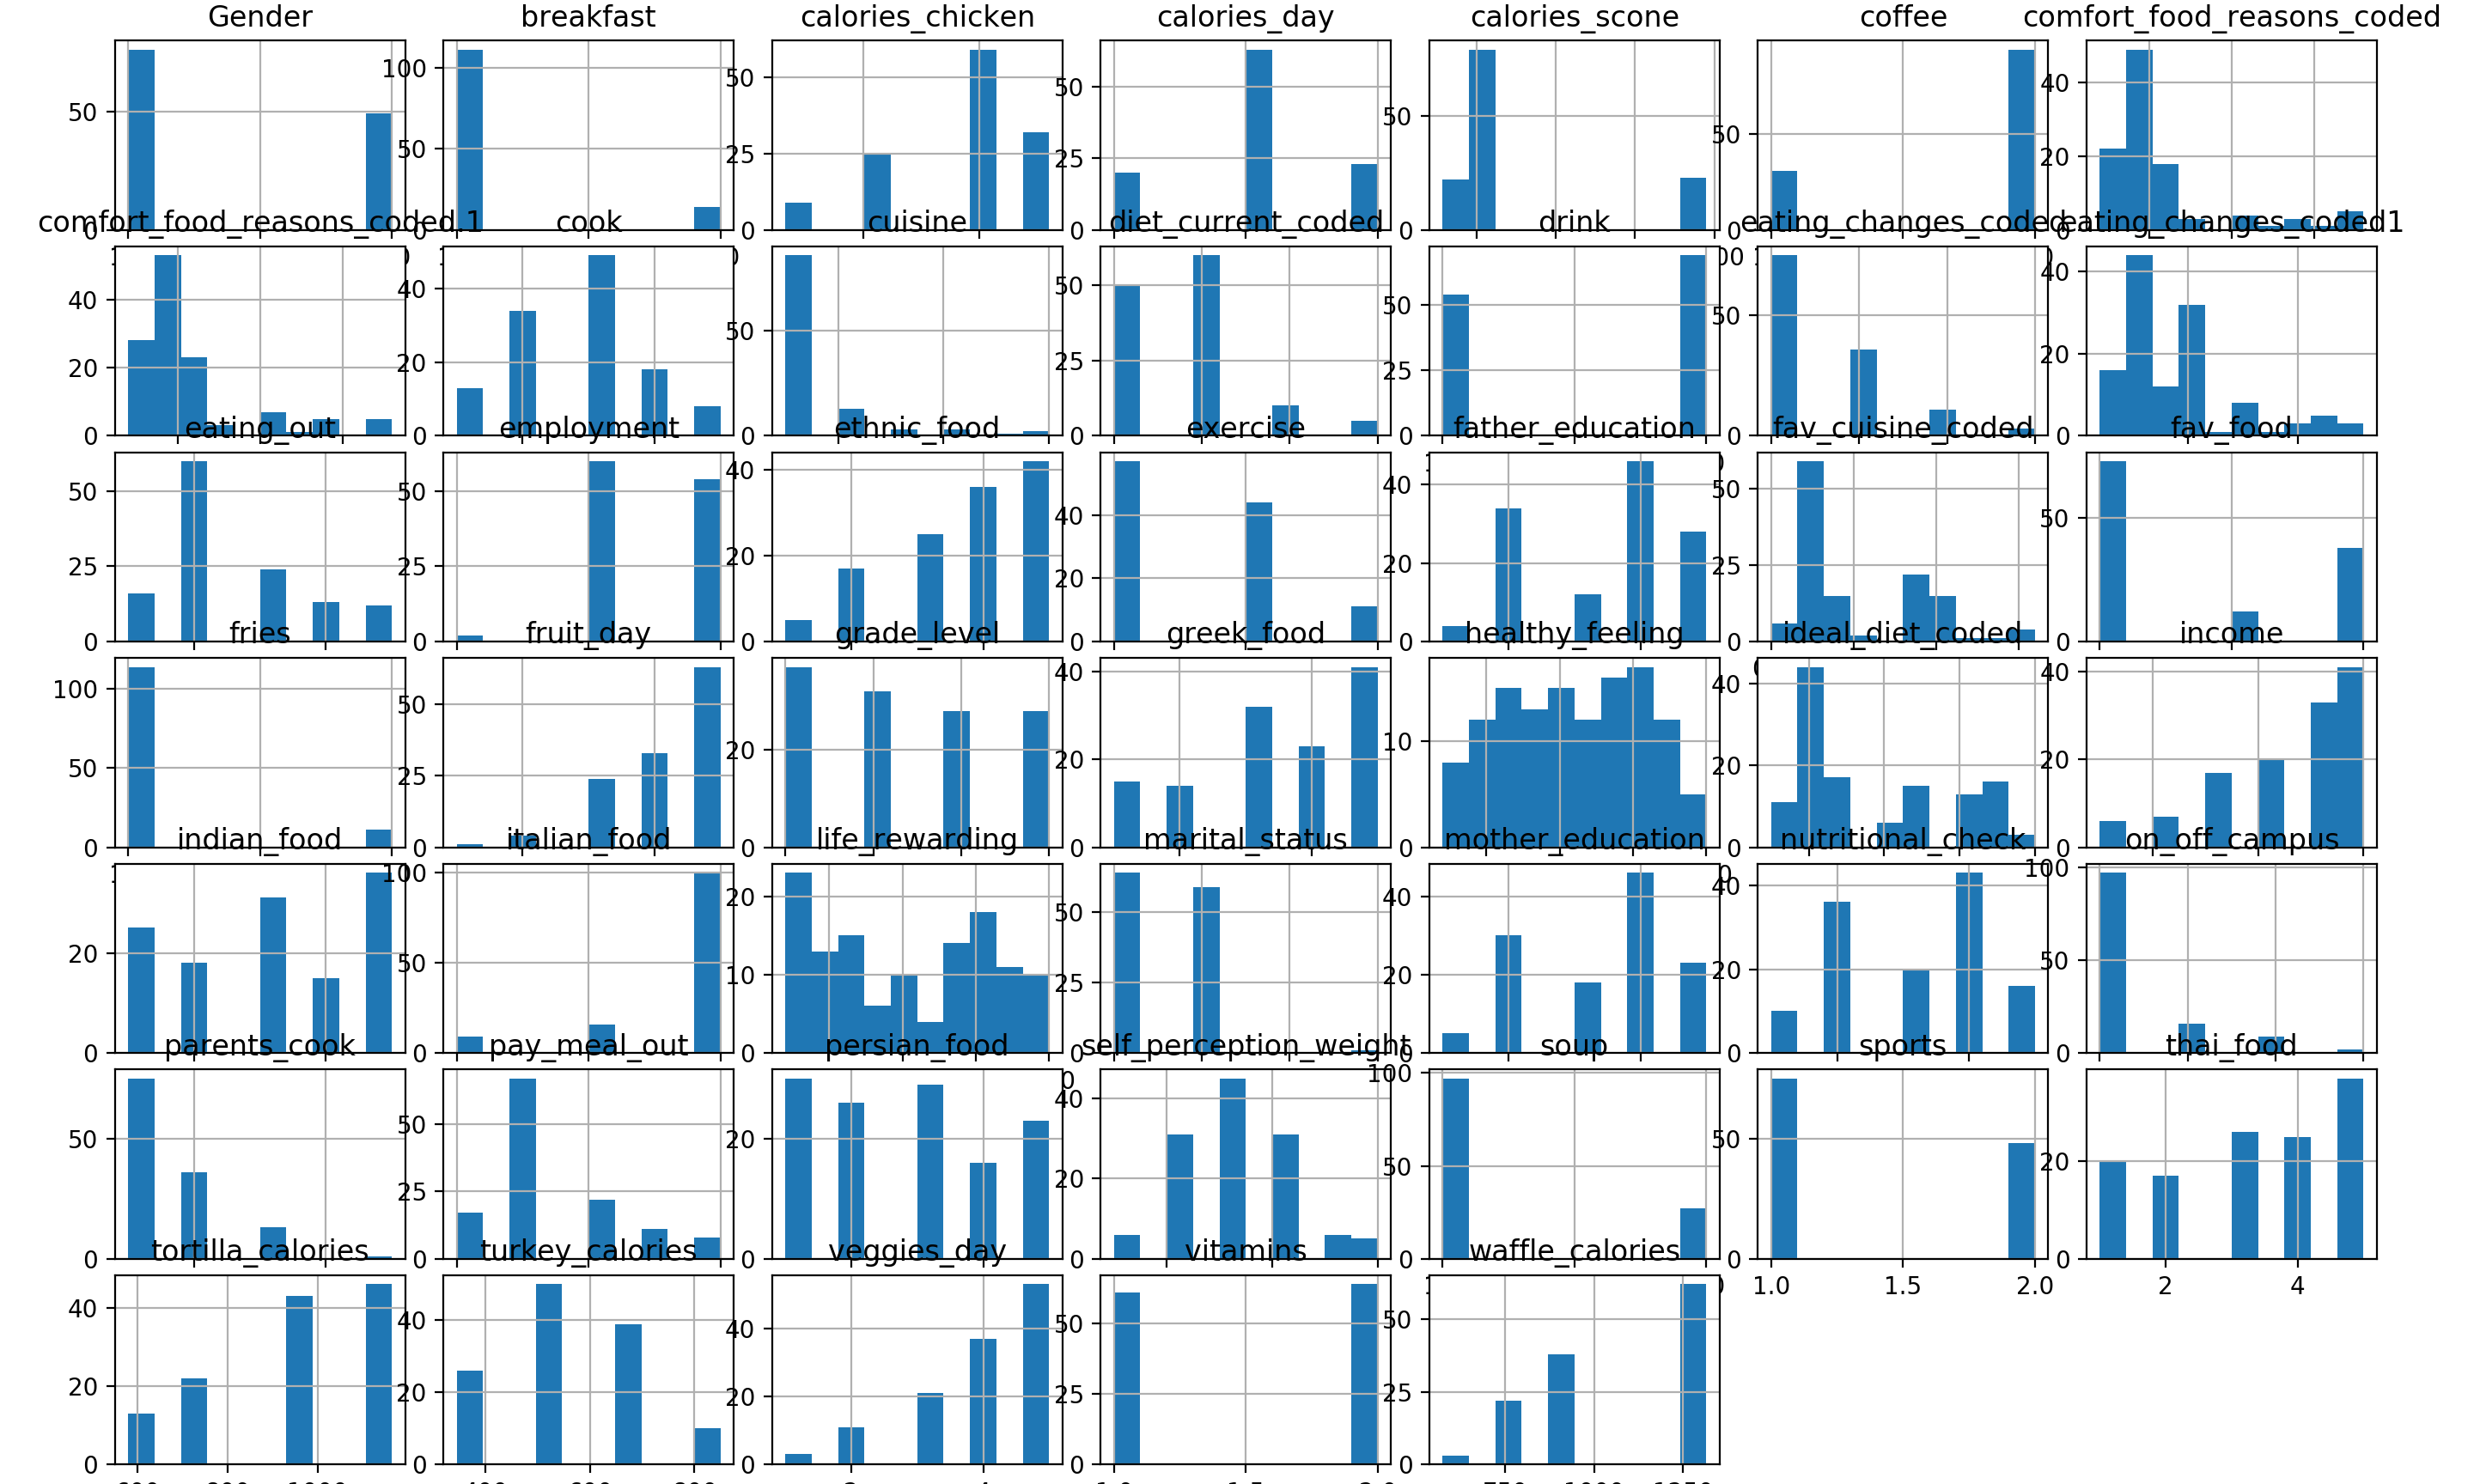
\includegraphics[width=15cm]{hist.png}
\end{figure}

Na osnovu histograma se jednostavno zaklju\v cuje da ima mnogo vi\v se \ zena, na primer. Za pitanja - atribute, koja su oblika "Od ponu\dj ene dve slike izabrati...", lako se mo\v ze dobiti odgovor \v sta su ljudi odgovarali u proseku. \\
Tako, velika ve\' cina njih je na pitanje \v sta za njih predstavlja doru\v cak odgovorila sa "\v zitarice", velika ve\' cina njih misli da je umereno va\v zno koliko se kalorija unosi dnevno. Veliki broj ispitanika svoju omiljenu hranu jede iz dosade, zbog stresa i depresije, dok zanemarljiv broj njih jede zbog gladi (\v sto bi trebalo da je glavni razlog zbog koga konzumiramo hranu). Tako\dj e, ve\' cina njih se bavi fizi\v ckom aktivno\v s\' cu. Na osnovu nekoliko histograma, mo\v ze se videti da je veliki broj ispitanika ljubitelj italijanske hrane: paste, testenina, pice, dok jako veliki broj njih ne bi okusilo indijsku hranu.

\newpage

\section{Primer klasifikacije}

Klasifikova\' cemo podatke na osnovu atributa comfort\_food\_reasons\_coded, cook i eating\_out, dok \' ce nam ciljni atribut biti weight.\\

\begin{lstlisting}[mathescape=true]
# najpre cemo ucitati podatke i prikazati prvih pet redova

df = pd.read_csv('./food-choices/food_coded.csv')
print('\n{}'.format(df.head()))
\end{lstlisting}

\begin{verbatim}
  GPA  Gender  breakfast ... waffle_calories                    weight
0   2.4       2          1 ...            1315                       187
1 3.654       1          1 ...             900                       155
2   3.3       1          1 ...             900  I'm not answering this.
3   3.2       1          1 ...            1315             Not sure, 240
4   3.5       1          1 ...             760                       190
\end{verbatim}

Mo\v zemo uraditi osnovnu statistiku za svaku kolonu.

\begin{lstlisting}[mathescape=true]
print("\nStatistike skupa:\n{}".format(df.describe()))
\end{lstlisting}

\begin{verbatim}
Statistike skupa:
           Gender   breakfast  calories_chicken ... veggies_day    vitamins
count  125.000000  125.000000        125.000000 ...  125.000000  125.000000
mean     1.392000    1.112000        577.320000 ...    4.008000    1.512000
std      0.490161    0.316636        131.214156 ...    1.081337    0.501867
min      1.000000    1.000000        265.000000 ...    1.000000    1.000000
25%      1.000000    1.000000        430.000000 ...    3.000000    1.000000
50%      1.000000    1.000000        610.000000 ...    4.000000    2.000000
75%      2.000000    1.000000        720.000000 ...    5.000000    2.000000
max      2.000000    2.000000        720.000000 ...    5.000000    2.000000
\end{verbatim}

Za algoritam koji \v zelimo da primenimo, izdvoji\' cemo slede\' ce atribute: comfort\_food\_reasons\_coded, cook, eating\_out i weight.

\begin{lstlisting}[mathescape=true]
target_attribute = 'weight'
attribute_1 = 'comfort_food_reasons_coded'
attribute_2 = 'cook'
attribute_3 = 'eating_out'

df = df[[attribute_1, attribute_2, attribute_3, target_attribute]]
\end{lstlisting}

\begin{verbatim}
   comfort_food_reasons_coded  cook  eating_out                    weight
0                         9.0   2.0           3                       187
1                         1.0   3.0           2                       155
2                         1.0   1.0           2  I'm not answering this.
3                         2.0   2.0           2             Not sure, 240
4                         1.0   1.0           2                       190
\end{verbatim}

Kao \v sto mo\v zemo primetiti, nisu sve vrednosti celobrojne. Zato \' cemo obrisati sve redove koji sadr\v ze NaN-ove ili niske u nekoj od ove \v cetiri kolone. Tako\dj e, vrednosti u koloni weight \' cemo transformisati. Preslika\' cemo ih u skup $\{0, 1, 2\}$. Dakle, \v zelimo da klasifikujemo ispitanike po te\v zini, u 3 grupe, u zavisnosti od toga koliko se \v cesto prejedaju, koliko \v cesto kuvaju i za\v sto jedu hranu za utehu. U prvu grupu spadaju oni koji su te\v ski do 150 funti (oko 70kg), u drugu oni koji imaju izme\dj u 70kg i 90 kg i u tre\' cu grupu oni sa preko 90kg.
\\ \\
Prvo se bri\v su nedostaju\' ce vrednosti.

\begin{lstlisting}[mathescape=true]
df = df.replace('nan', np.nan)
df = df.dropna()


df = df[df[target_attribute].apply(lambda x: str(x).isdigit())]

df.reset_index(drop=True, inplace=True)

df[attribute_1] = df.comfort_food_reasons_coded.astype(int)
df[attribute_2] = df.cook.astype(int)
df[attribute_3] = df.eating_out.astype(int)
df[target_attribute] = df.weight.astype(int)

changes = {}
weight = df[target_attribute].unique()
for w in weight:
    if int(w) < 150:
        changes[w] = 0
    elif int(w) < 190:
        changes[w] = 1
    else:
        changes[w] = 2

df[target_attribute] = df[target_attribute].replace(changes)
\end{lstlisting}

\begin{verbatim}
   comfort_food_reasons_coded  cook  eating_out  weight
0                           9     2           3       1
1                           1     3           2       1
2                           1     1           2       2
3                           4     3           1       2
4                           1     2           2       1
\end{verbatim}

Sada \' cemo izvr\v siti podelu skupa na test i trening skup.

\begin{lstlisting}
X = df[[attribute_1, attribute_2, attribute_3]]
y = df[[target_attribute]]

X_train, X_test, y_train, y_test = train_test_split(X, y, test_size=0.3)
print("\nVelicina skupa za obucavanje: {}".format(X_train.size))
print("Velicina skupa za testiranje: {}".format(X_test.size))
\end{lstlisting}

\begin{verbatim}
Velicina skupa za obucavanje: 207
Velicina skupa za testiranje: 90
\end{verbatim}

Po\v sto smo izvr\v sili podelu skupa, primeni\' cemo algoritam za klasifikaciju - $k$ najbli\v zih suseda.

\begin{lstlisting}
clf = KNeighborsClassifier(5, 'distance')

# Treniramo model
clf.fit(X_train, y_train.values.ravel())

# Vrsimo predikciju
y_test_predicted = clf.predict(X_test)
y_train_predicted = clf.predict(X_train)

# Izracunavamo preciznost
train_acc = clf.score(X_train, y_train)
test_acc = clf.score(X_test, y_test)
print('train preciznost: {}'.format(train_acc))
print('test preciznost: {}'.format(test_acc))
\end{lstlisting}

\begin{verbatim}
train preciznost: 0.7536231884057971
test preciznost: 0.7
\end{verbatim}

Izve\v staj i matricu konfuzije mo\v zemo dobiti na slede\' ci na\v cin:

\begin{lstlisting}
test_rep = sklearn.metrics.classification_report(y_test, y_test_predicted)
train_rep = sklearn.metrics.classification_report(y_train, y_train_predicted)
print("\nTest izvestaj:\n{}".format(test_rep))
print("Trening izvestaj:\n{}".format(train_rep))

train_conf = sklearn.metrics.confusion_matrix(y_train, y_train_predicted)
test_conf = sklearn.metrics.confusion_matrix(y_test, y_test_predicted)
print("Matrica konfuzije za skup za obucavanje:\n{}".format(train_conf))
print("\nMatrica konfuzije za skup za testiranje:\n{}".format(test_conf))
\end{lstlisting}

\begin{verbatim}
Test izvestaj:
             precision    recall  f1-score   support

          0       0.67      0.91      0.77        11
          1       0.77      0.67      0.71        15
          2       0.50      0.25      0.33         4

avg / total       0.70      0.70      0.68        30

Trening izvestaj:
             precision    recall  f1-score   support

          0       0.74      0.86      0.79        29
          1       0.73      0.81      0.77        27
          2       1.00      0.38      0.56        13

avg / total       0.78      0.75      0.74        69

Matrica konfuzije za skup za obucavanje:
[[25  4  0]
 [ 5 22  0]
 [ 4  4  5]]

Matrica konfuzije za skup za testiranje:
[[10  1  0]
 [ 4 10  1]
 [ 1  2  1]]
\end{verbatim}

Kao \v sto se mo\v ze videti iz matrica konfuzije za test i trening skup, podaci su dosta dobro klasifikovani - broj ta\v cno klasifikovanih je dosta veliki, za razliku od onih koji to nisu.

\newpage

\section{Vizuelizacija podataka}

Atributi koje posmatramo:
\begin{itemize}
  \item self\_perception\_weight\\
    procena sopstvene te\v zine
  \item fruit\_day\\
    Koliko je verovatno da bi pojeli vo\' ce u toku dana
  \item pay\_meal\_out\\
    Koliko bi platili za jedan obrok?
   \item weight\\
     Te\v zina
\end{itemize}

\begin{lstlisting}
import pandas as pd
import matplotlib.pyplot as plt
import numpy as np
from mpl_toolkits.mplot3d import Axes3D

# read data
df = pd.read_csv('./food-choices/food_coded.csv')

# choose attributes
target_attribute = 'weight'
attribute_1 = 'self_perception_weight'
attribute_2 = 'fruit_day'
attribute_3 = 'pay_meal_out'

df = df[[attribute_1, attribute_2, attribute_3, target_attribute]]

# data preprocessing

# remove NaN
df = df.replace('nan', np.nan)
df = df.dropna()

df = df[df[target_attribute].apply(lambda x: str(x).isdigit())]

df.reset_index(drop=True, inplace=True)

df[attribute_1] = df.self_perception_weight.astype(int)
df[attribute_2] = df.fruit_day.astype(int)
df[attribute_3] = df.pay_meal_out.astype(int)
df[target_attribute] = df.weight.astype(int)

# transform target attribute
changes = {}
weight = df[target_attribute].unique()
for w in weight:
    if int(w) <=128:
        changes[w] = 0
    elif int(w) <= 155:
        changes[w] = 1
    elif int(w) <= 180:
        changes[w] = 2
    else:
        changes[w] = 3

df[target_attribute] = df[target_attribute].replace(changes)
weight = df[target_attribute].unique()

fig = plt.figure()
ax = fig.add_subplot(111, projection='3d')

colors = ['green','blue','orange','red']
for (v, color) in zip(weight, colors):
    subsamples = df.loc[df[target_attribute] == v]
    ax.scatter(subsamples[attribute_1], 
               subsamples[attribute_2],
               subsamples[attribute_3],
               color=color,s=70,alpha=0.3)

ax.set_xlabel('self_perception_weight')
ax.set_ylabel('fruit_day')
ax.set_zlabel('pay_meal_out')
plt.show()
\end{lstlisting}

\begin{figure}[H]
  \centering
  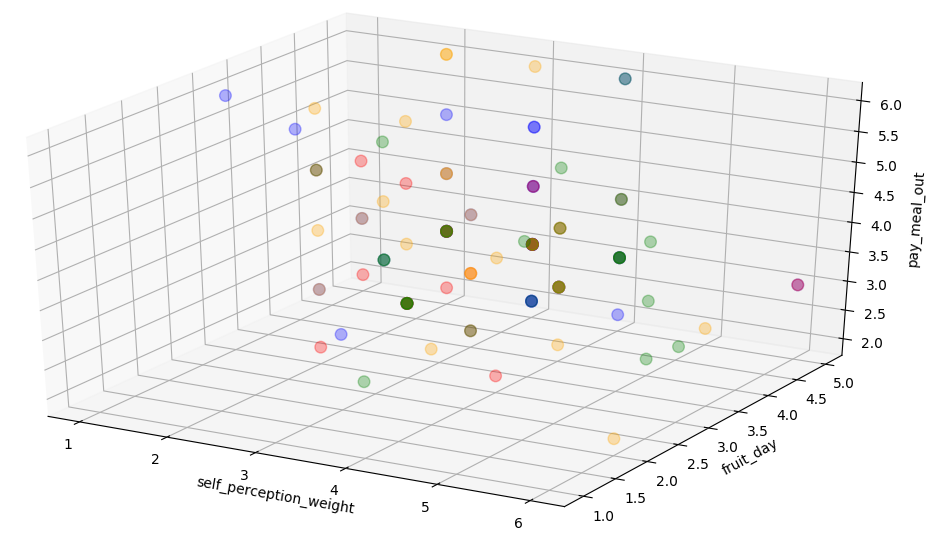
\includegraphics[width=15cm]{3dgrafik.png}
\end{figure}

\subsection{PCA}

\lstset{language=python,
     xleftmargin=20pt,
      basicstyle=\ttfamily,
      morekeywords={to, downto, then},
      keywordstyle=\color{blue}\ttfamily,
      stringstyle=\color{red}\ttfamily,
      commentstyle=\color{green}\ttfamily,
      morecomment=[l][\color{magenta}]{\#},
      numbers=none,
      basicstyle=\small
}

Kori\v s\' cenjem PCA algoritma \' cemo redukovati skup na manji, zadr\v zavaju\' ci ve\' cinu informacija iz inicijalnog skupa podataka.

\begin{lstlisting}
from sklearn.decomposition import PCA
import pandas as pd
import matplotlib.pyplot as plt
import numpy as np
from sklearn.preprocessing import StandardScaler

def isFloat(value):
  try:
    float(value)
    return True
  except ValueError:
    return False

df = pd.read_csv('./food-choices/food_coded.csv')

# odabir atributa

target_attribute = 'weight'
attributes = [ 'exercise','Gender','eating_out',
               'GPA','employment','breakfast', 
               'calories_chicken','calories_day','coffee',
               'diet_current_coded','drink','cook']

df = df[[attributes[0],attributes[1],attributes[2],
         attributes[3],attributes[4],attributes[5],
         attributes[6],attributes[7],attributes[8],
         attributes[9],attributes[10],attributes[11],
         target_attribute]]

# obrada podataka
# brisanje redova sa nedostajucim vrednostima,
# konvertovanje podataka u odgovarajuce
# kako bi se moglo raditi sa njima

df = df.replace('nan', np.nan)
df = df.dropna()

df = df[df[target_attribute].apply(lambda x: str(x).isdigit())]
df = df[df['GPA'].apply(lambda x: isFloat(str(x)))]

df.reset_index(drop=True, inplace=True)

# podaci su tipa float, a potrebno je
# da budu tipa int, pa se u narednim
# koracima vrsi konverzija

df[attributes[0]] = df.exercise.astype(int)
df[attributes[1]] = df.Gender.astype(int)
df[attributes[2]] = df.eating_out.astype(int)
df[attributes[3]] = df.GPA.astype(float)
df[attributes[4]] = df.employment.astype(int)
df[attributes[5]] = df.breakfast.astype(int)
df[attributes[6]] = df.calories_chicken.astype(int)
df[attributes[7]] = df.calories_day.astype(int)
df[attributes[8]] = df.coffee.astype(int)
df[attributes[9]] = df.diet_current_coded.astype(int)
df[attributes[10]] = df.drink.astype(int)
df[attributes[11]] = df.cook.astype(int)
df[target_attribute] = df.weight.astype(int)

# transformisanje ciljnog atributa
# preslikacemo sve vrednosti weight atributa
# u skup {0, 1, 2, 3}
# ispitanici:
# sa manje od 58.5kg spadaju u grupu 0
# izmedju 58.5 i 70kg spadaju u grupu 1
# izmedju 70 i 81.6kg spadaju u grupu 2
# sa preko 81.6kg spadaju u grupu 3

changes = {}
weight = df[target_attribute].unique()

for w in weight:
    if int(w) <=128:
        changes[w] = 0
    elif int(w) <= 155:
        changes[w] = 1
    elif int(w) <= 180:
        changes[w] = 2
    else:
        changes[w] = 3

df[target_attribute] = df[target_attribute].replace(changes)
weight = df[target_attribute].unique()

features = attributes 

# extract features
x = df.loc[:, features].values
# extract target attribute
y = df.loc[:,[target_attribute]].values

x = StandardScaler().fit_transform(x)

pca = PCA(n_components=2)
principalComponents = pca.fit_transform(x)
principalDf = pd.DataFrame(data = principalComponents
             ,columns=['principal component 1','principal component 2'])

finalDf = pd.concat([principalDf,df[[target_attribute]]],axis = 1)

fig = plt.figure(figsize = (8,8))
ax = fig.add_subplot(1,1,1) 
ax.set_xlabel('Principal Component 1',fontsize = 15)
ax.set_ylabel('Principal Component 2',fontsize = 15)
ax.set_title('2 component PCA', fontsize = 20)

targets = [0,1,2,3]
colors = ['green','blue','orange','red']
for target, color in zip(targets,colors):
    indicesToKeep = finalDf[target_attribute] == target
    ax.scatter(finalDf.loc[indicesToKeep,'principal component 1']
              ,finalDf.loc[indicesToKeep,'principal component 2']
              ,c=color
              ,s=50)

ax.legend(['0-128', '129-155','156-180','180+'])
ax.grid()
plt.show()
\end{lstlisting}

\begin{figure}[H]
  \centering
  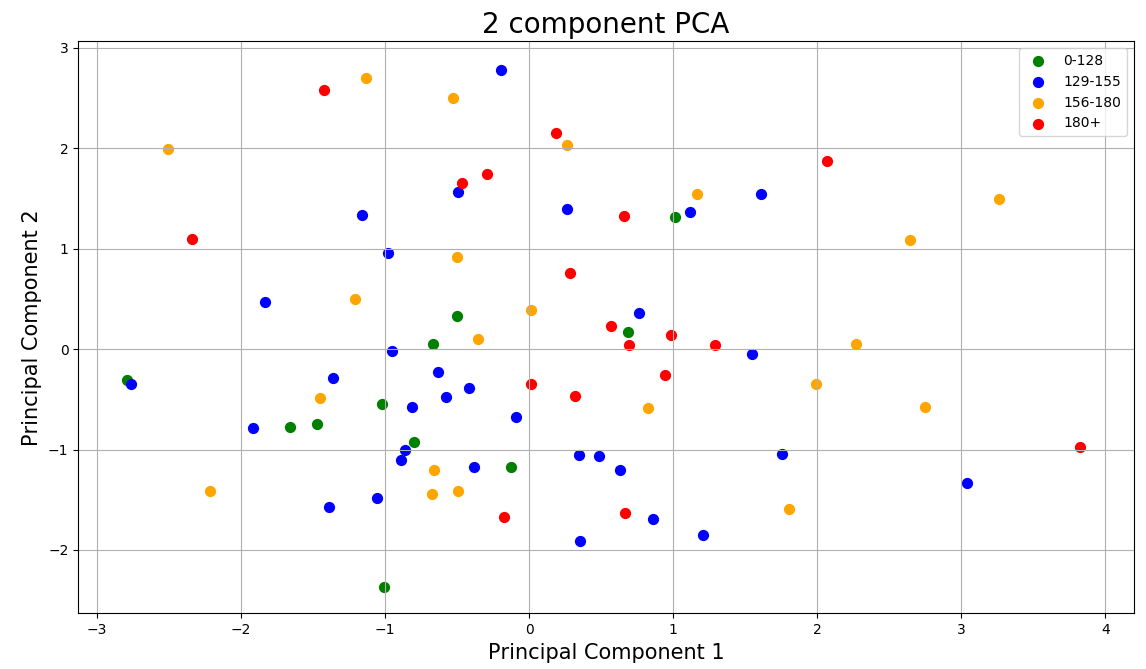
\includegraphics[width=15cm]{pca.png}
\end{figure}

Na osnovu grafika zaklju\v cujemo da najve\' ci broj ispitanika ima izme\dj u 58.5kg i 70kg.

\end{document}
